\documentclass[10pt,twocolumn,letterpaper]{article}

\usepackage{cvpr}
\usepackage{times}
\usepackage{epsfig}
\usepackage{graphicx}
\usepackage{amsmath}
\usepackage{amssymb}

% Include other packages here, before hyperref.

% If you comment hyperref and then uncomment it, you should delete
% egpaper.aux before re-running latex.  (Or just hit 'q' on the first latex
% run, let it finish, and you should be clear).
\usepackage[breaklinks=true,bookmarks=false]{hyperref}

\cvprfinalcopy % *** Uncomment this line for the final submission

\def\cvprPaperID{****} % *** Enter the CVPR Paper ID here
\def\httilde{\mbox{\tt\raisebox{-.5ex}{\symbol{126}}}}

% Pages are numbered in submission mode, and unnumbered in camera-ready
%\ifcvprfinal\pagestyle{empty}\fi
% \setcounter{page}{4321}
\begin{document}

%%%%%%%%% TITLE
\title{Pushbroom satellite image super-resolution using generative adversarial networks}

\author{Chao Xu\\
The Chinese University of Hong Kong\\
Shatin, New Territories, Hong Kong SAR\\
{\tt\small 1155160618@lin.cuhk.edu.hk}
% For a paper whose authors are all at the same institution,
% omit the following lines up until the closing ``}''.
% Additional authors and addresses can be added with ``\and'',
% just like the second author.
% To save space, use either the email address or home page, not both
}
\maketitle
%\thispagestyle{empty}

%%%%%%%%% ABSTRACT
\begin{abstract}
In order to improve the resolution or visual effect of imageries from pushbroom sensors, this report proposes to use super-resolution generative adversarial networks (SRGAN)~\cite{ledig2017photo}. Some improvements are achieved: firstly, the VGG-19~\cite{simonyan2014very} network is modified to extract the features of input images, and thus reduce the training time; secondly, the loss function is updated as new evaluation metric for the generated images; finally, three models with different hyperparameters are trained and compared to find the optimal results. In this report,  the pushbroom image super-resolution is achieved with a scale factor of 4, and the result shows a better visual perception compared with that recovered by bicubic interpolation. We call the network model in this report as pbiSRGAN, which is Push-Broom Images SRGAN.         
\end{abstract}

%%%%%%%%% BODY TEXT
\section{Introduction}
Pushbroom imaging has been one of the most common satellite scanning methods over the past decades, which features in low manufacturing cost and relatively high maneuvering~\cite{chao2020study}.  However, its spatial resolution is usually degraded due to strong atmospheric turbulences, fierce temperature fluctuation or the Earth rotation, \etal. As the development of CMOS and CCD technology, the size of single detector pixel is getting smaller and the density of detector array is increasing, which help improve the satellite image resolution but also greatly level up the hardware manufacturing cost. Therefore, software methods such as imaging super-resolution algorithms have been proposed recently.

Conventional super-resolution methods include nonuniform interpolation, maximum a posteriori, projection on convex sets, and iterative back projection~\cite{park2003super}. These  methods have their own constraints, such as multiple solutions, instability or image blurring. Since the beginning of this decade, deep learning has been keeping advancing itself into various areas, including object detection, image classification, speech recognition and so on.  Imaging super-resolution has been a hot topic in the deep learning community since it is first introduced in 2015 as SRCNN~\cite{dong2015image}. In 2017, a perceptual loss is additional proposed in SRGAN~\cite{ledig2017photo} as a complement to the conventional pixel-based loss metrics, and it is another landmark in the area of deep learning image super-resolution. Essentially, the SRGAN method is also a variant of GAN proposed in 2014~\cite{goodfellow2014generative}.

In this report, we will first talk about the basic principle of SRGAN, which is different from those methods generating images pixelwisely, but creates more visually perceptual images with high resolution.  Secondly, a neural network architecture for pushbroom images is described, including how it is fit for gray-scale remote sensing imageries, how to reduce training time and improve training efficiency. Finally, three experimental groups will be set up with different hyper-parameters to find the optimal results for the pbiSRGAN.
%-------------------------------------------------------------------------
\section{Key concept of SRGAN}
%To understand how SRGAN works, we first need to understand the classic network model GAN, which laid an important foundation for its subsequent variants. Here, we will not list the complex mathematical formulas in GAN, but illustrate the meaning of GAN by a simple example.  As the name suggests, G stands for generative network, and can be considered as a criminal who produces counterfeit money. On the other hand, D, as a discriminator,  is the bank's note examiner, who specializes in checking whether the money made by G is fake or real. At first, G's ability to fake money was very poor, and could be easily checked out by D. After each failure, G carefully gained the experience and constantly improved his ability to fake money. In this way, D gradually found it difficult to distinguish the real money from the fake one, and then D also began to improve his ability to check counterfeit money, and summed up his experience of wrong judgment. Finally, over and over again, the power of both the generator and the discriminator are improved.

As for SRGAN, the low-resolution images are fed into the generation network and "high-resolution images" are generated as the input of the discriminant network. The discriminator needs to determine whether the input images are  generated "high-resolution image" or the original ground truth value. The super resolution process is completed when the equal probabilities are obtained of "high-resolution images" being  judged as true or false.  At this time, the generative network can be used to generate the "high-resolution images" closest to the ground truth value. Here, it is also necessary to mention the way of "summarizing experience" for both networks, namely, loss function. The loss function used in SRGAN is critical to the final network, which is different from the traditional per-pixelwise MSE loss. It evaluates the generated image from the perspective of human visual perception~\cite{ledig2017photo}. The advantage of pixelwise MSE loss is that it achieves a very high PSNR, but the reconstructed images are lack of high-frequency information, resulting in over-smooth image texture and poor visual effect. Specifically, the perceptual loss function $L^{SR}$ is composed of content loss $L_{Con}^{SR}$ and weighted generative loss $L_{Gen}^{SR}$:
\begin{equation}\label{eq1}
{L^{SR}} = \underbrace {\underbrace {L_{\text{Con}}^{SR}}_{{\text{ content loss }}} + \underbrace {{{10}^{ - 3}}L_{{\text{Gen}}}^{SR}}_{{\text{ generative loss }}}}_{{\text{perceptual loss}}}
\end{equation}

Content loss uses VGG-19~\cite{simonyan2014very} as the feature extractor of the input image. The pre-trained network has strong feature extraction capability. Content loss is defined as the Euclidean distance between the reconstructed image $G{\left(I^{L R}\right)}$ and the reference image $I^{HR}$ feature map:
\begin{equation}\label{eq2}
L_{Con}^{SR} = \sum\limits_{x = 1}^{{W_{i,j}}} {\sum\limits_{y = 1}^{{H_{i,j}}} {{{\left( {{\phi _{i,j}}{{\left( {{I^{HR}}} \right)}_{x,y}},{\phi _{i,j}}{{\left( {G\left( {{I^{LR}}} \right)} \right)}_{x,y}}} \right)}^2}} } 
\end{equation}
where $W_{I,j}$ and $H_{I,j}$ respectively represent the dimensions of each feature map in VGG-19 network; ${\phi _{i,j}}$ refers to the feature map \cite{ledig2017photo} obtained by the convolution layer $j$ in front of the max pooling layer $i$ in VGG-19 network.

The other part of the perceptual loss is generative loss, which makes the generated results more consistent with the real images of human visual perception.
\begin{equation}\label{eq3}
L_{Gen}^{SR} = \sum\limits_{n = 1}^N { - \log D\left( {G\left( {{I^{LR}}} \right)} \right)} 
\end{equation}
where $D{\left(G\left(I^{L R}\right)\right)}$ is defined as the probability that the discriminator D determines the reconstructed images as real high resolution images, and $N$ is the number of generated samples.

\section{From SRGAN to pbiSRGAN}
Compared with natural images, there is a serious problem applying SRGAN to remote sensing pushbroom images, that is, the lack of real training sets containing high-low resolution image pairs. Specifically, if the real image obtained by the satellite is regarded as a low-resolution image, and then it is impossible to obtain the corresponding ground truth as a high-resolution image. It is obvious that the satellite cannot avoid atmospheric turbulence, temperature fluctuation and other factors in the real-scene shooting, therefore, it is impossible to obtain a higher resolution image. The only way to get high-low resolution image pair is to take the real satellite image as a high-resolution image (i.e., ground truth) and then simulate a low-resolution version of it. In addition, SRGAN is originally proposed to solve the super-resolution problem of naturally colorful images, and can not be directly used for remote sensing data. Remote sensing images can be divided into panchromatic, multispectral, hyperspectral and even hyperspectral data, whose image channels range from one to hundreds. The remote sensing imageries own the characteristics of large scanning scale and great data volume, and the coverage of a single shot can reach dozens or even hundreds of square kilometers. Therefore, we proposed pbiSRGAN to achieve the purpose of super-resolution for pushbroom scanning remote sensing images.

\section{Training and reconstructing of pbiSRGAN}
The section aim to training and reconstructing process of remote sensing image super-resolution. 
\subsection{pbiSRGAN training flow}
The training flowchart is shown in Fig.~\ref{fig1} for model of pbiSRGAN.

In the first step,  a panchromatic remote sensing image used and preprocessed to make it as the initial ground truth of network input. The steps of preprocessing include histogram equalization and random cutting. The former aims to improve the contrast of the image and is beneficial to the extraction of the feature map. The latter is to generate sufficient data sets, including training sets, validation sets, and testing sets.

Second, after the training set enters the network, bicubic interpolation with a certain scale factor is conducted to generate the corresponding low-resolution images (namely, the high-resolution images are downsampled), and thus obtaining the HR and LR image pairs in the training process.

The third step is to train the generative network G. The low-resolution image LR is passed through G to get "generated high-resolution image" $G{\left(I^{L R}\right)}$. Since the network G is weak at first, the quality of $G{\left(I^{L R}\right)}$ may not be as good as LR. Here, we need to evaluate the loss of the generated image. The loss of the network G $L_{G}^{SR}$ is mainly divided into two parts, namely the content loss $L_{Con}^{SR} $ and generative loss $L_{Gen} ^{SR}$. $L_{Con}^{SR}$ is evaluated by Eq.(\ref{eq4}):
\begin{equation}\label{eq4}
L_{Con}^{SR} = \sum\limits_{x = 1}^{{W_{i,j}}} {\sum\limits_{y = 1}^{{H_{i,j}}} {{{\left\| {{\phi _{i,j}}{{\left( {{I^{HR}}} \right)}_{x,y}},{\phi _{i,j}}{{\left( {G\left( {{I^{LR}}} \right)} \right)}_{x,y}}} \right\|}_1}} } 
\end{equation} 
That is, the feature maps of $G{\left(I^{LR}\right)}$ and HR are extracted through the modified VGG-19 network, and the $L_1$ distance between them is calculated. The $L_2$ norm is mainly related with the Gaussian distribution error, while the $L_1$ norm is related to the Laplace error. When the image contains non-Gaussian errors, the confidence of $L_1$ norm is higher than that of $L_2$ norm~\cite{song2010adaptive}. Only when the error of the model is Gaussian white noise distribution, the solution of $L_2$ model is optimal, which is difficult to achieve in real world. 

$L_{Gen}^{SR}$ is also redesigned as shown in Eq.(\ref{eq5}):
\begin{equation}\label{eq5}
L_{Gen}^{SR} = \sum\limits_{n = 1}^N {{\rm{1}} - \log D\left( {G\left( {{I^{LR}}} \right)} \right)} 
\end{equation}

Finally, we need to train the discriminator D. The power of network D can be strengthened by iteration of the loss function $L_{D}^{SR}$, which consists of two parts,  $L_{real}^{SR}$ to discriminate $I^{HR}$ as true and $L_{fake}^{SR}$ to discriminate $G{\left(I^{L R}\right)}$ as false.
\begin{equation}\label{eq7}
L_{real}^{SR} = \sum\limits_{n = 1}^N {{\rm{1}} - \log D\left( {{I^{HR}}} \right)}
\end{equation}

\begin{equation}\label{eq8}
L_{fake}^{SR} = \sum\limits_{n = 1}^N { - \log D\left( {G\left( {{I^{LR}}} \right)} \right)}
\end{equation}

\begin{equation}\label{eq9}
L_D^{SR} = \frac{1}{2}\left( {L_{real}^{SR} + L_{fake}^{SR}} \right)
\end{equation}

\subsection{pbiSRGAN reconstructing flow}
While validating the generative networks using validation set, super-resolution reconstruction can also be accomplished, as shown in Fig.~\ref{fig2}.

\section{Network architecture of pbiSRGAN}
The network is mainly divided into three parts: feature extraction network F, generative network G and discriminant network D.
\subsection{Feature extraction network}
The basic prototype of the feature extraction network comes from the VGG-19 network, which is a 19-layer pre-training network with very strong feature extraction ability, but it cannot be directly applied to the network model in this project. VGG-19 is used for feature extraction of colorful images. In this section, the previous 18 layers of VGG-19 are extracted, and the first layer of VGG-19 is modified into a structure suitable for single-channel gray remote sensing images. In this way, the feature extraction network F can obtain the corresponding features from the ground truth value and generated images, and then carry out loss calculation. The structure of network F is shown in Fig.~\ref{fig3}.

\subsection{Generative network}
Generative network G is the core of the whole pbiSRGAN network, which will generate high-resolution images. The network structure we designed is shown in the Fig.~\ref{fig4}, the core of which is the residual block. The role of residual blocks will be discussed later.

Specifically, a convolution layer with kernel size of $9 \ times 9$ is used first, and the input is a single-channel low-resolution image and the output is a 64-channel feature map. A Parametric Rectified Linear Unit (PRELU) is then used as the activation function, with the parameter of . As shown in Fig.~\ref{eq5}, PRELU is actually a variant of Leaky Rectified Linear Unit (Lrelu). For LReLU, if $x<0, y=0.01x$;For PReLU, if $x<0$, then $y=ax$. Compared with ReLU, the advantages of using PReLU are to prevent zero activation of the network and speed up the training process.

Next, we use 16 residuals blocks, all of which have the same structure. Using residuals blocks helps solve the optimization problem when the forward network is too deep~\cite{gross2016training}. The structure of each residual block is shown in Fig.~\ref{fig6}. Its first layer is a convolution layer, with input and output channels of 64, and the size of the convolution kernel is $3 \ times 3$. What follows up is a batch normalization (BN) layer that speeds up training by reducing covariance shifts within the dataset, allowing us to use larger learning rates during training without decreasing output quality\cite{ioffe2015batch}. After activation by PRELU, there is another pair of convolution layer and batch normalization layer with the same parameters as above, and the final output is 64-channel feature map.

As shown in the Fig.~\ref{fig4}, after passing the output of the PReLU1 layer and the 16 residual blocks to the BN33 layer, we used two trained sub-pixel convolution layers to increase the resolution of the input image~\cite{shi2016real}. The core of the sub-pixel convolution layer is the PixelShuffle layer, which can convert the 4-dimensional data in the training process from $(*,C\times r\times r,H,W)$ to $(*,C,H\times r,W\times r)$, where $*$ represents the batch size of the data set. $C$, $H$ and $W$ are the dimension of the images, and $r$ is the scale factor. Finally, the generated high-resolution image is obtained through the Conv37 layer.

\subsection{Discriminant network}
The main function of discriminant network D is to battle with generative network G, so as to improve the power of G. The discriminant network designed in this project is shown in the Fig.~\ref{fig7}, with a total of 24 layers.The initial input channel and the final output channel are both designed as 1. In addition, the convolution layer of 64, 128, 256 and 512 channels is designed to gradually improve the feature extraction ability. The detailed parameters can be seen in the table ~\ref{tab1}.



Please direct any questions to the production editor in charge of these 
proceedings at the IEEE Computer Society Press: 
\url{https://www.computer.org/about/contact}. 


{\small
\bibliographystyle{ieee_fullname}
\bibliography{egbib}
}



\begin{figure*}
\begin{center}
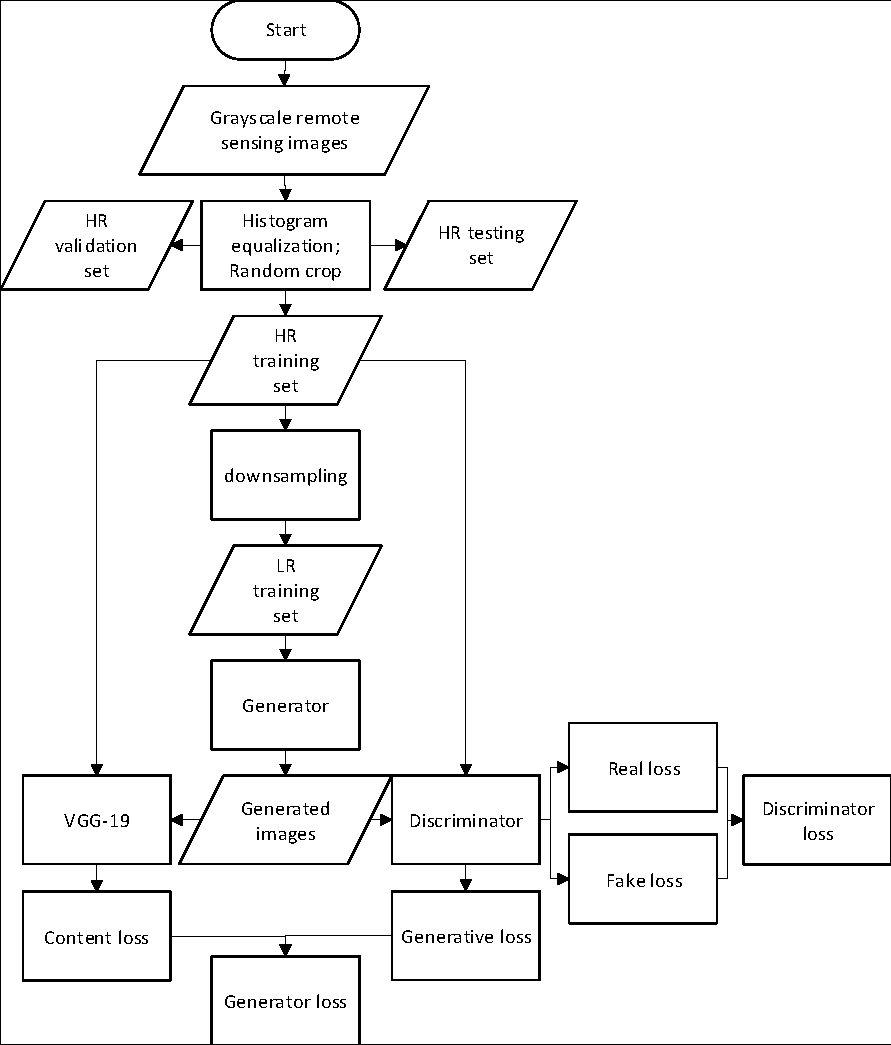
\includegraphics[width=0.8\textwidth]{fig1}
\end{center}
   \caption{Training flow chart of pbiSRGAN.}
\label{fig1}
\end{figure*}

 \begin{figure*}
\begin{center}
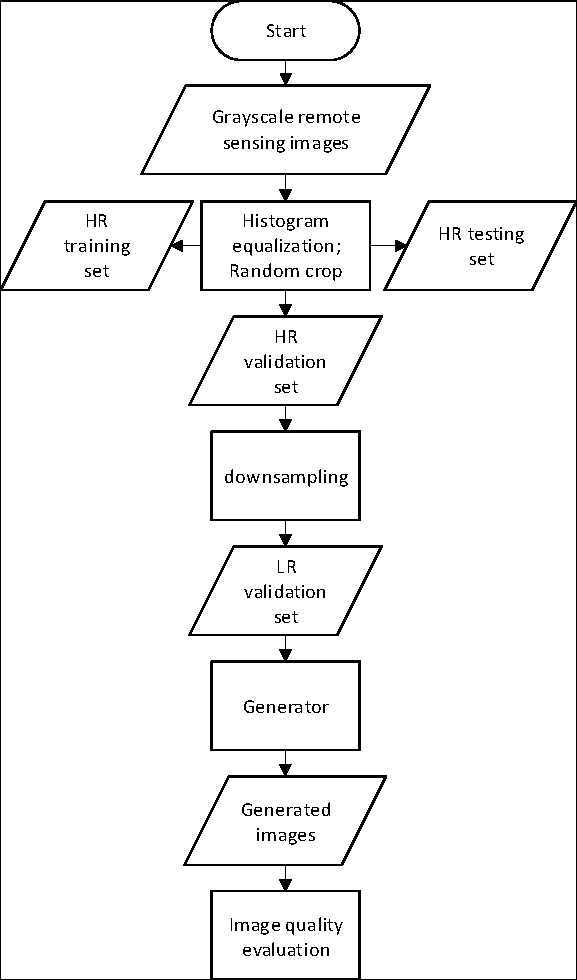
\includegraphics[width=0.5\textwidth]{fig2}
\end{center}
   \caption{Reconstructing flow chart of pbiSRGAN.}
\label{fig2}
\end{figure*}

 \begin{figure*}
\begin{center}
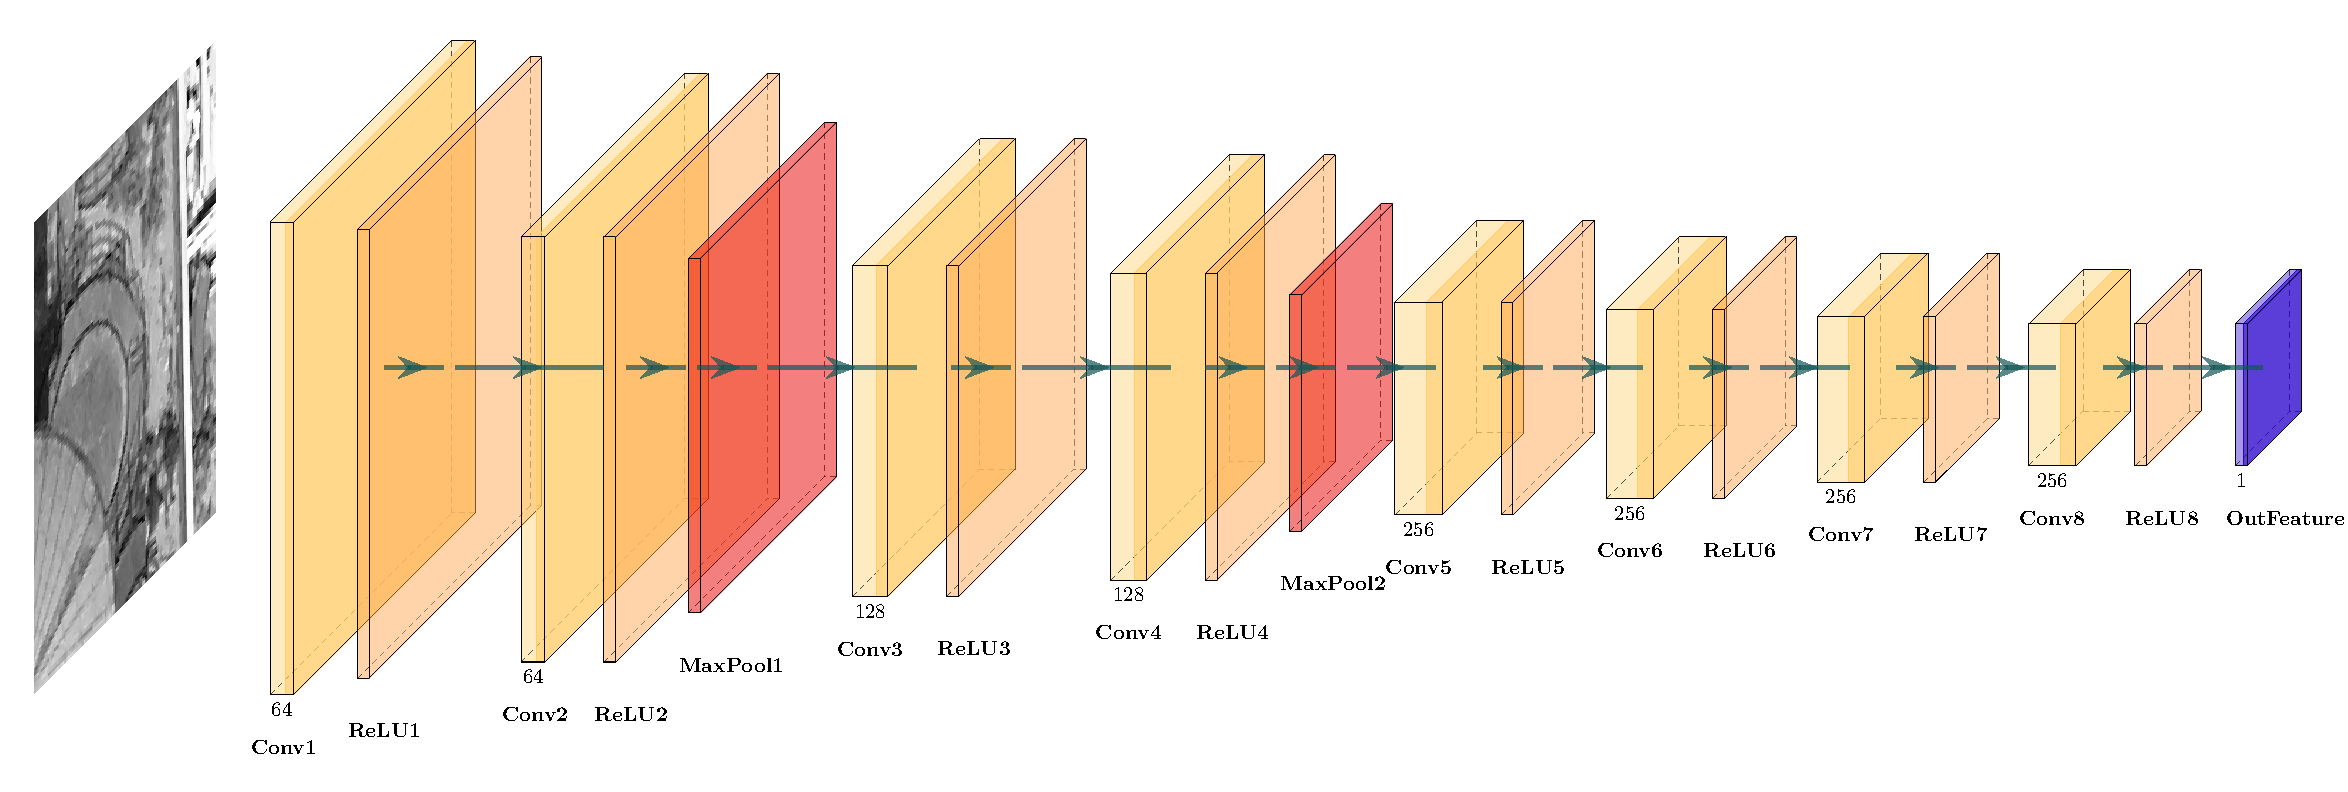
\includegraphics[width=1\textwidth]{fig3}
\end{center}
   \caption{Architecture of feature extractor network.}
\label{fig3}
\end{figure*}

 \begin{figure*}
\begin{center}
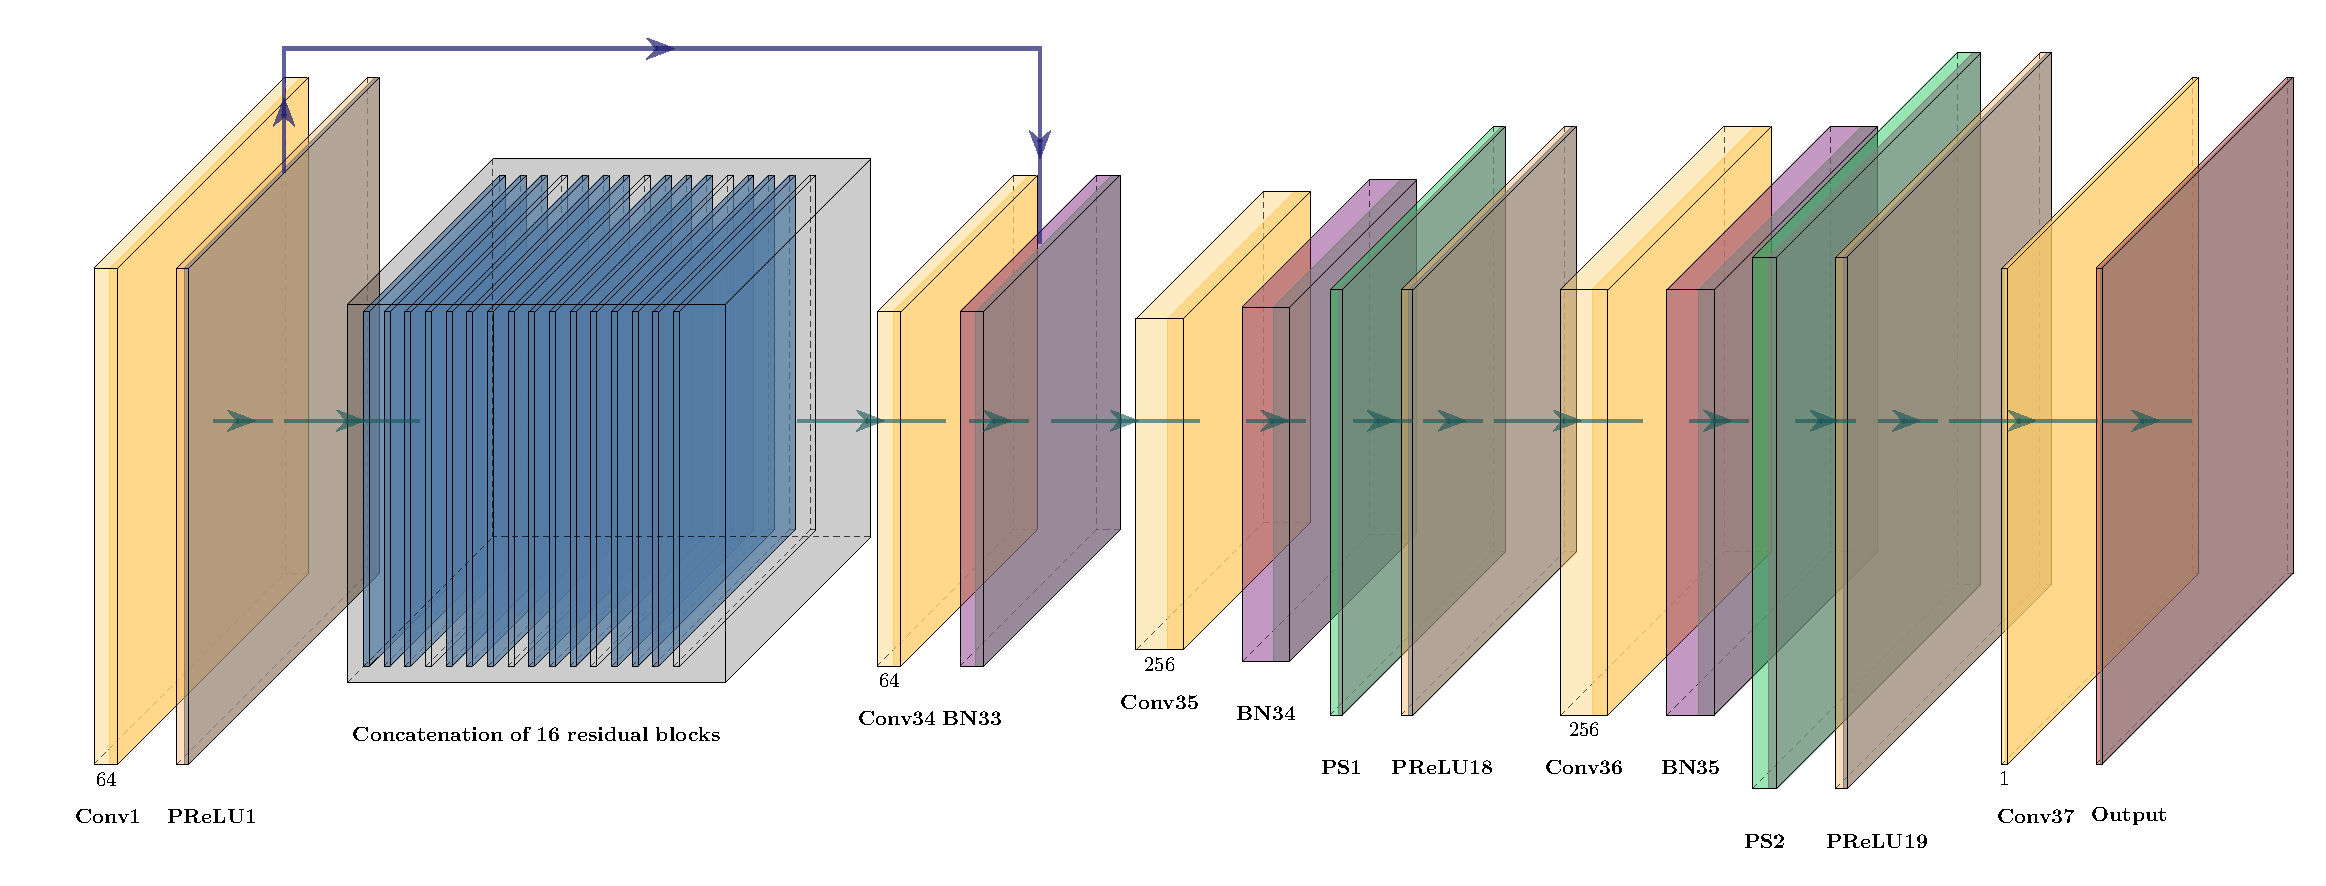
\includegraphics[width=1\textwidth]{fig4}
\end{center}
   \caption{Architecture of generative network.}
\label{fig4}
\end{figure*}

 \begin{figure*}
\begin{center}
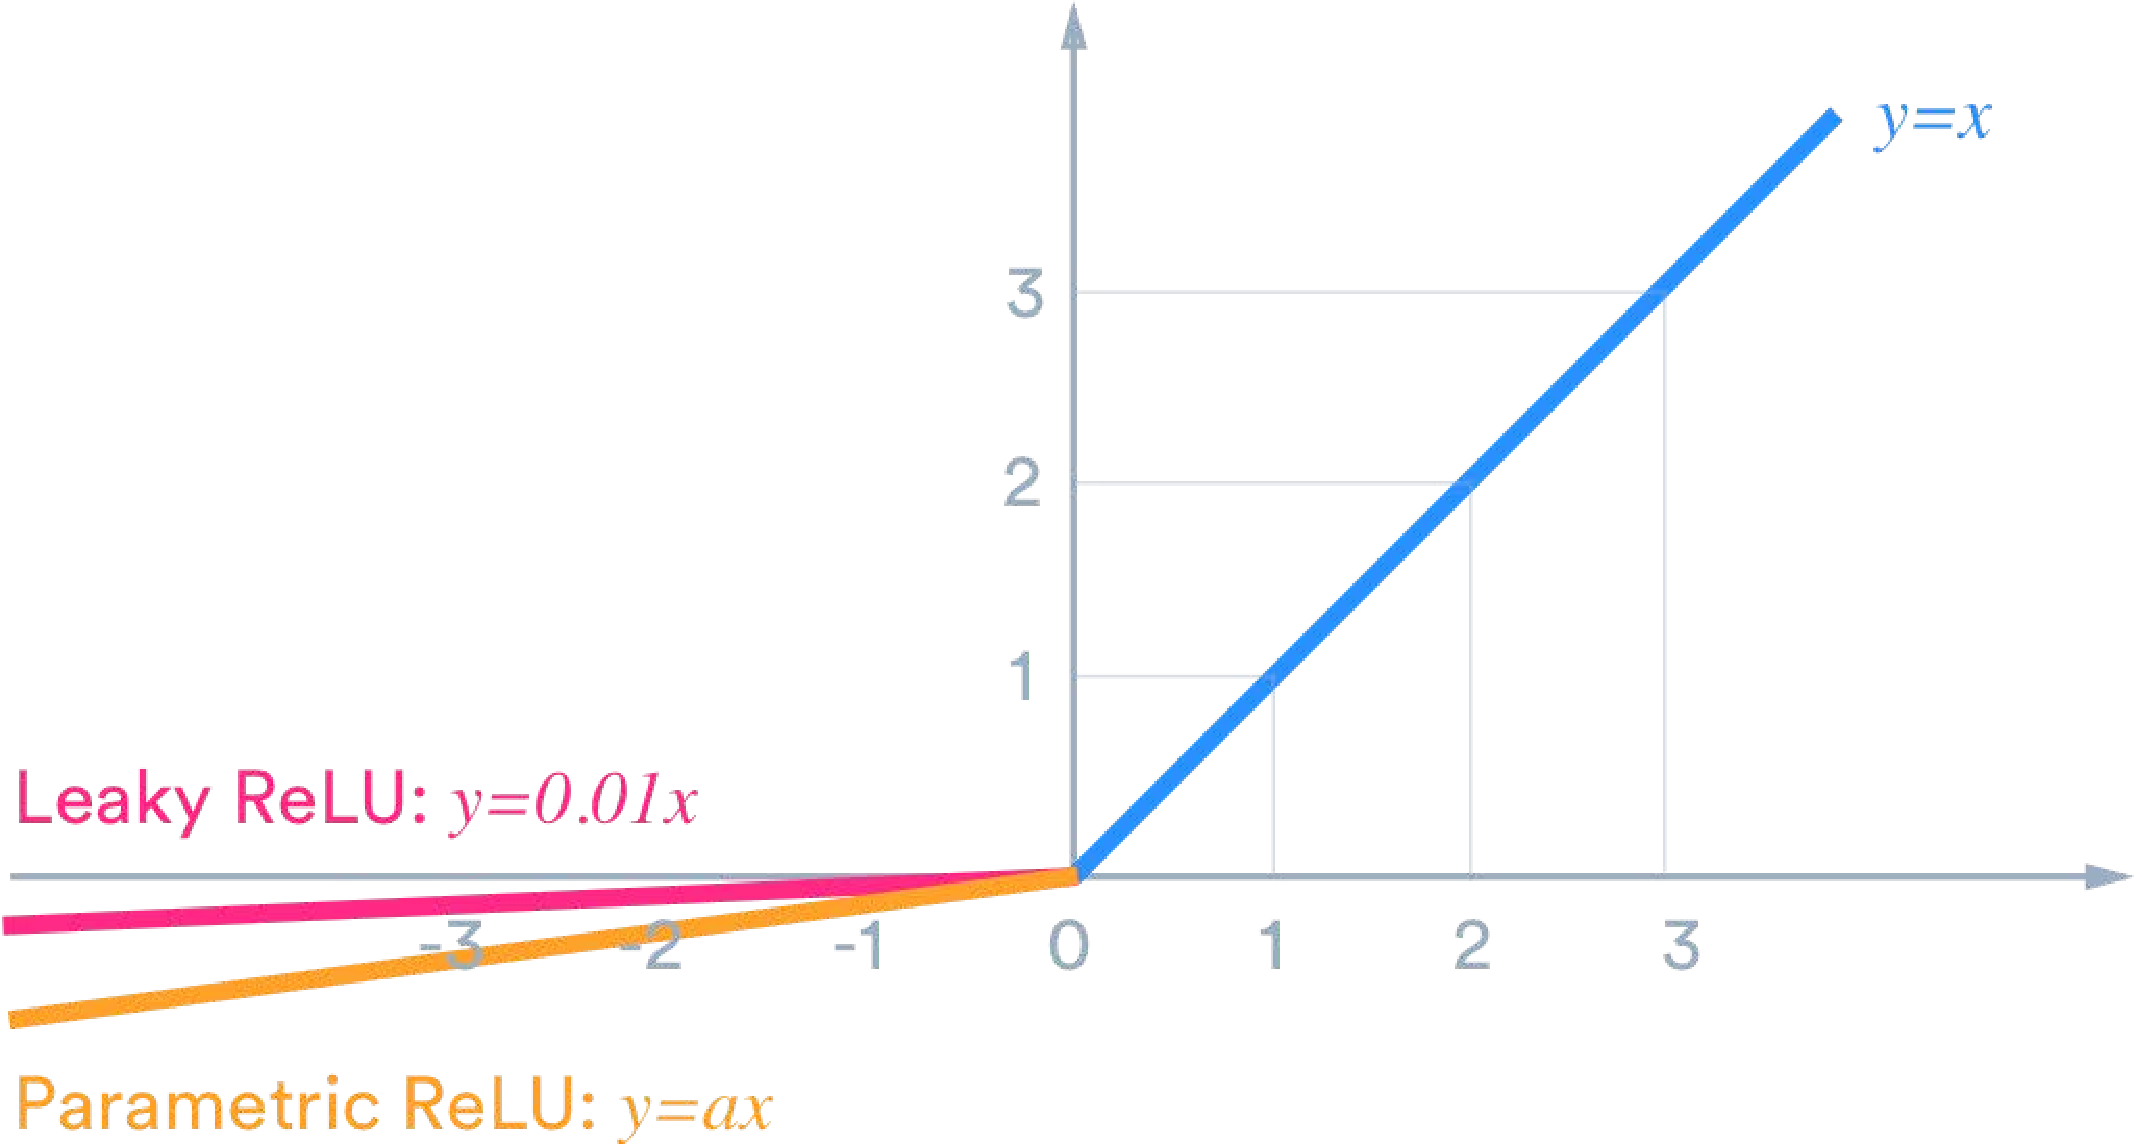
\includegraphics[width=1\textwidth]{fig5}
\end{center}
   \caption{Representation of LReLU and PReLU.}
\label{fig5}
\end{figure*}

 \begin{figure*}
\begin{center}
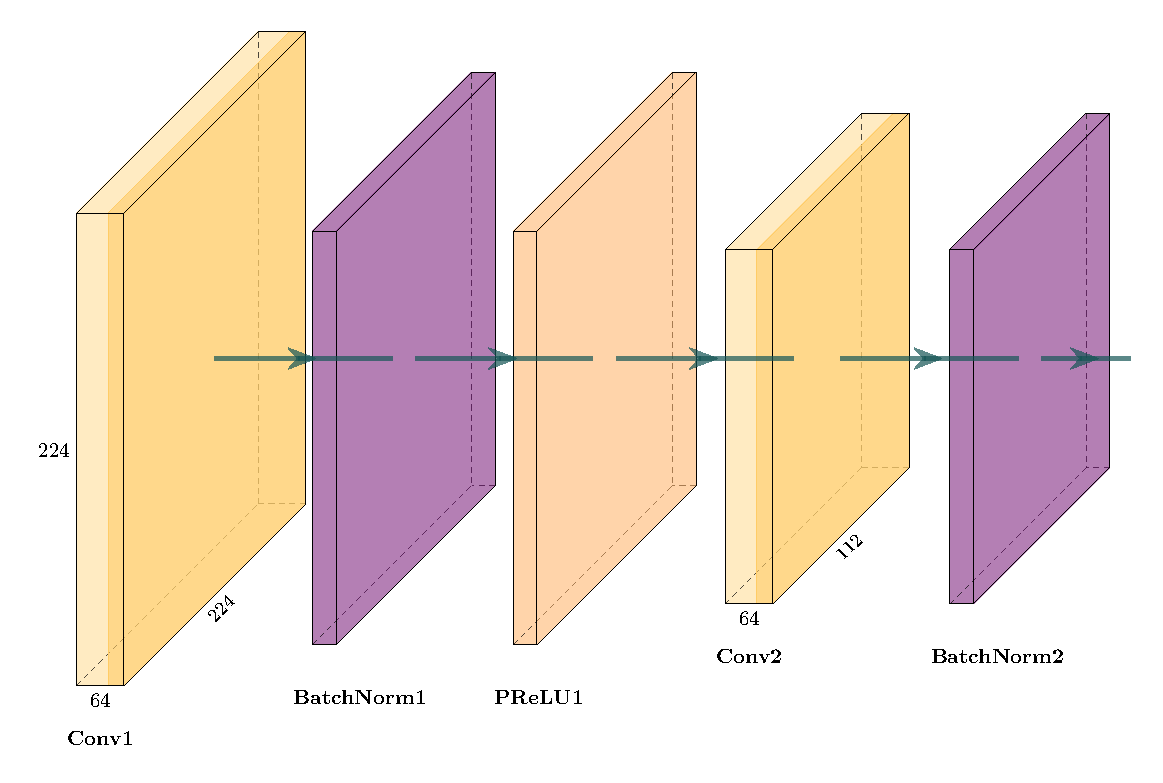
\includegraphics[width=1\textwidth]{fig6}
\end{center}
   \caption{Architecture of residual block.}
\label{fig6}
\end{figure*}

 \begin{figure*}
\begin{center}
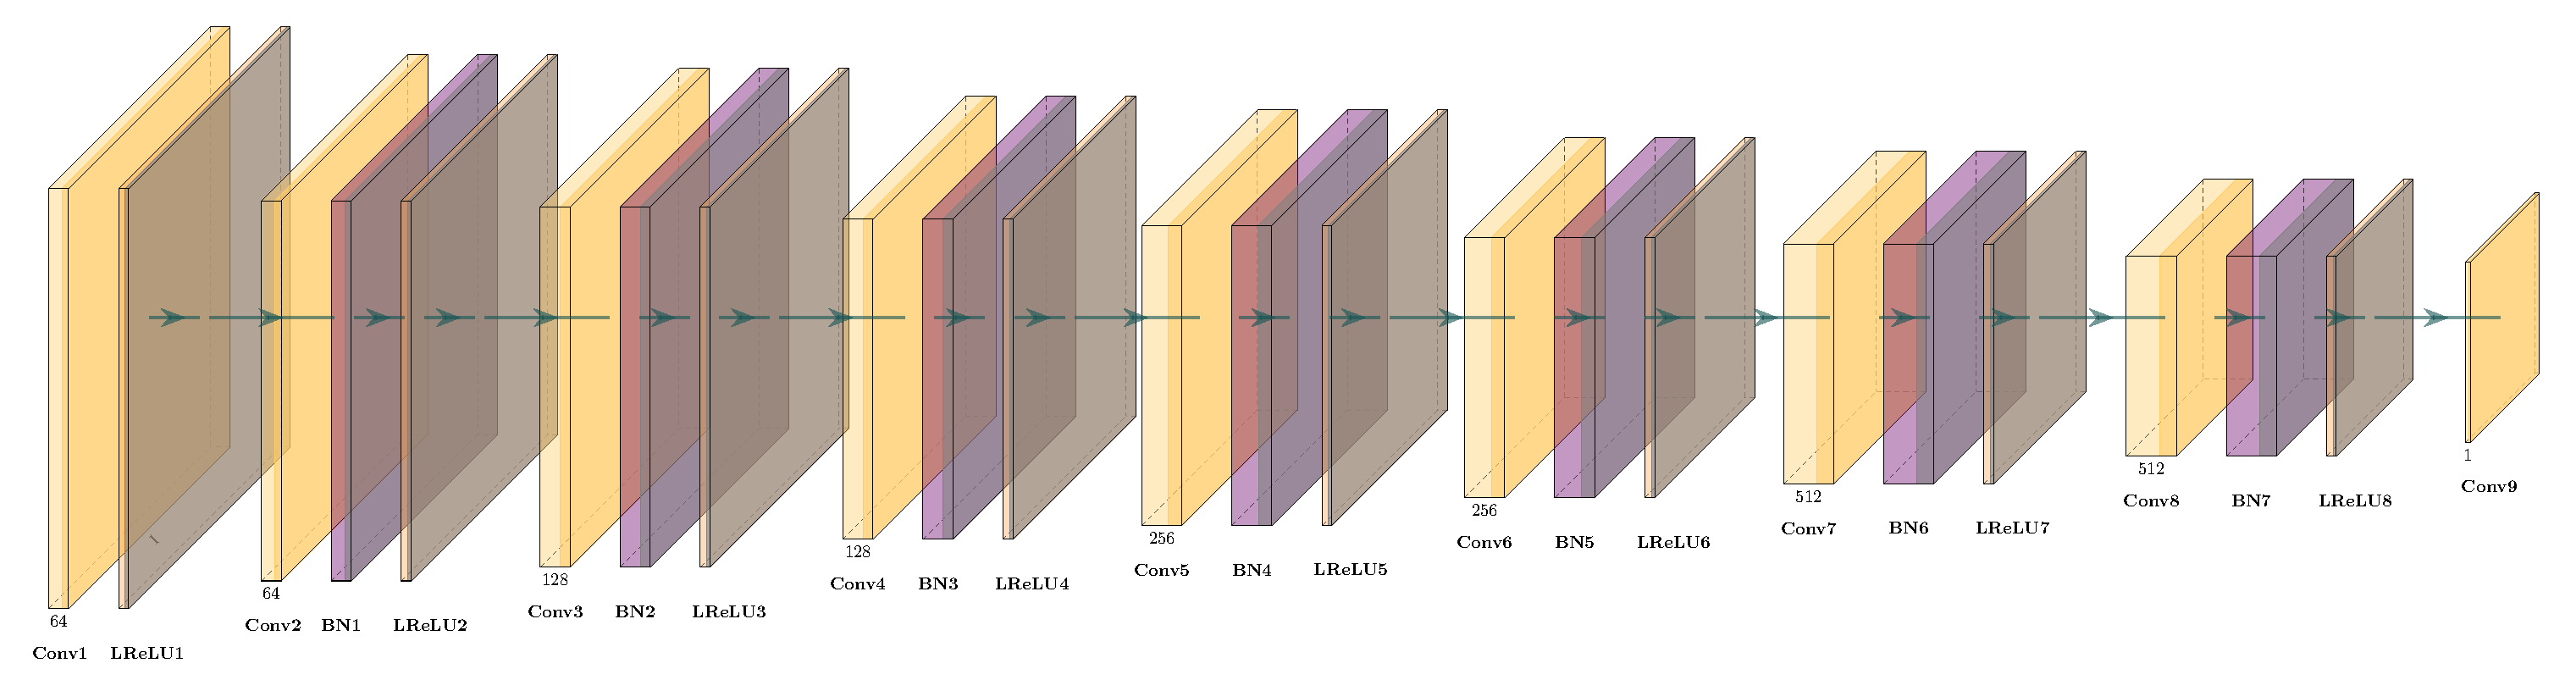
\includegraphics[width=1\textwidth]{fig7}
\end{center}
   \caption{Architecture of discriminator network.}
\label{fig7}
\end{figure*}

\begin{table}
\begin{center}
	\begin{tabular}{lccc}
		\hline		
		No.&Layer      &Input channel&Output channe\\
		\hline
		1  &Conv2d     &1        &64    \\
		2  &LeakyReLU  &-        &-       \\
		3  &Conv2d     &64       &64     	\\
		4  &BatchNorm2d&64       &64    \\
		5  &LeakyReLU  &-        &-        \\
		6  &Conv2d     &64       &128       \\
		7  &BatchNorm2d&128      &128      \\
		8  &LeakyReLU  &-        &-        \\
		9  &Conv2d     &128      &128     \\
		10 &BatchNorm2d&128      &128      \\
		11 &LeakyReLU  &-        &-      \\
		12 &Conv2d     &128      &256     \\
		13 &BatchNorm2d&256      &256 \\
		14 &LeakyReLU  &-        &-      \\
		15 &Conv2d     &256      &256     \\
		16 &BatchNorm2d&256      &256     \\
		17 &LeakyReLU  &-        &-       \\
		18 &Conv2d     &256      &512     \\
		19 &BatchNorm2d&512      &512     \\
		20 &LeakyReLU  &-        &-       \\
		21 &Conv2d     &512      &512     \\
		22 &BatchNorm2d&512      &512     \\
		23 &LeakyReLU  &-        &-       \\
		24 &Conv2d     &512      &1       \\
		\hline
	\end{tabular}
\end{center}
\caption{Parameters of discriminant network.}
\label{tab1}
\end{table}



\end{document}
